\setchapterpreamble[u]{\margintoc}
\chapter{Evaluating discretization approaches for ultralight structure optimization}
The process of topology optimization for a structure involves the selection and sizing of optimal elements within a predetermined set. As discussed in the previous chapter, in our context this set could be composed of either continuum elements (shell or volumetric) or truss-like elements. This chapter aims to assess the suitability and the inherent advantages and disadvantages of both methodologies when optimizing ultralight structures \ie structures that exhibit \marginnote{Part of the content presented in this chapter has been published and showcased during a conference as:\\Stragiotti, E. et al. (2021) "Towards manufactured lattice structures: a comparison between layout and topology optimization", in \textit{AeroBest 2021 International Conference on Multidisciplinary Design Optimization of Aerospace Systems}. Book of proceedings. Lisbon, Portugal: ECCOMAS~\cite{stragiotti_towards_2021}.} an extremely low volume fraction, typically below 1\%. 

For this purpose, we initially establish a common optimization formulation in \secref{sec:03_common_prob}. The classic compliance minimization with volume constraint problem is reformulated as a volume minimization problem with maximum stress constraints for both discretization. Later, this framework is applied to optimize a two-dimensional test case, featuring identical dimensions, loads, and material properties. The outcomes of the comparison of both discretization approaches are presented and discussed in \secref{sec:03_comparison}. 

\section{The formulation of a common problem: volume minimization with stress constraints} \label{sec:03_common_prob}
Two of the most frequently employed formulations for structural optimization are the minimization of volume while adhering to stress constraints and the minimization of compliance under volume constraints. Historically, the volume minimization formulation has been used in the first works of structural optimization of truss structures~\sidecite{dorn_automatic_1964,chan_optimum_1964,hemp_optimum_1973}. The problem was initially formulated in terms of member forces, ignoring the kinematic compatibility to obtain a \gls{lp} problem. The formulation was modeled using the \acrfull{sand} approach, where the equations of nodal equilibrium are treated as equality constraints, and where both nodal displacements and the cross-sectional areas of truss members serve as design variables~\sidecite{sankaranarayanan_truss_1994}. 

However, to attain greater design freedom, the structure optimization field later transitioned from truss structures to continuous discretization. While truss structures offered simplicity and ease of analysis, they imposed limitations on design due to their discrete member configurations. The continuum mesh offered instead more versatility~\sidecite{bendsoe_generating_1988,bendsoe_optimal_1989}, and has since been used for multiple different applications, \eg the design of metamaterials~\sidecite{sigmund_materials_1994, zhang_scale-related_2006}. The \gls{sand} approach is incompatible with continuum meshes due to its excessive number of variables\sidenote{This preposition holds true when referring to the end of the 1980s, when computational power was scarce compared to what we have today.}. Given this limitation, a new approach was required to better handle the complexity of continuum meshes.

In the \acrfull{nand} approach, the nodal displacement (state) variables are eliminated from the optimization problem through a process where the structural equilibrium equation is solved every iteration instead of being used as a constraint of the optimization. This results in an independent nested phase where the state equation of structural equilibrium is solved separately from the optimization algorithm. This creates a dense coupling between displacement and material density variables, necessitating a computationally expensive sensitivity analysis within the nested algorithm, typically employing the adjoint method (more information about the adjoint method on the following resurces~\sidecite{tortorelli_design_1994,martins_engineering_2021}). Nevertheless, if the problem is reformulated as a compliance minimization with volume constraints, the problem is self-adjoint and the adjoint algorithm is no longer necessary to evaluate the gradient sensitivities~\sidecite{bendsoe_topology_2004}.

However, our emphasis on operating within the aerospace sector aligns more favorably with the volume minimization problem. The choice to prioritize volume minimization in the aerospace sector is underpinned by a range of economic, environmental, and performance-related factors. It is a strategic approach that aligns with industry goals of sustainability, efficiency, and technological advancement. Additionally, as we will see later in this thesis, the volume minimization formulation will permit adding local buckling and maximum displacements constraints in an easier way. We have opted, thus, to employ the volume minimization optimization formulation for our study, and we will now review how this formulation is implemented on continuum and truss-like meshes.

\subsection{Continuous discretization \gls{nand} minimum volume formulation}
This section introduces the \gls{nand} volume minimization formulation of topology optimization for continuum meshes. We will start however presenting the more common minimum compliance formulation to explain the important notations and concepts that will be essential in developing the volume minimization formulation.

\paragraph{Minimum compliance formulation}
\begin{marginfigure}
    \centering
    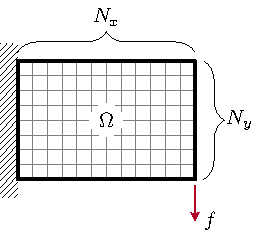
\includegraphics{figures/03_comparison_TO_TTO/00_contin_mesh/c_mesh.pdf}
    \caption{The domain $\Omega$ is discretized using $N_e=N_x N_y$ continuous 4-nodes elements.}
    \label{fig:03_mesh_c}
\end{marginfigure}
Let $\Omega \in \mathbb{R}^2$ be a rectangular domain in of dimensions $X$ and $Y$, containing respectively $N_x$ and $N_y$ linear 4-nodes elements, for a total of $N_e=N_x N_y$ elements and $M$ nodes (see \figref{fig:03_mesh_c}). The objective of the optimization is the minimization of the compliance $C$ of the structure, equivalent to finding the structure with the least possible nodal displacement with respect to a defined set of boundary conditions. The problem $\mathbb{T}_0$ is stated in terms of the design variables $\vect{\rho}$ as follows:
\begin{equation}
    \begin{aligned}
    \min_{\vect{\rho}}         && C &= \sum_{i} \vect{u}_{e,i}^T \matr{K}_{e,i} \vect{u}_{e,i}=\vect{f}^T\vect{u}&& \forall i \in [0,\dots,N_e]                         \\
    \textrm{s.t.}   && & \frac{\sum_{i} \left(\rhophys_i v_i \right) / V_0}{V^*} - 1 \leq 0 && \forall i \in [0,\dots,N_e] \\
    && \matr{K}\vect{u} &= \vect{f} &&\\
    && 0 &\leq \rho_i \leq 1. && \forall i \in [0,\dots,N_e] \\
    \end{aligned}
    \tag{$\mathbb{T}_0$}
    \label{eq:03_prob-comp}
\end{equation}
The design variables $\vect{\rho}$ are defined for every element of the structure as $\vect{\rho} = [\rho_1, \rho_2, \ldots,\rho_{Ne}]^T$, with $\rho_i \in [0,1], \; \forall i \in [0,\dots,N_e]$. The physical densities $\vect{\rhophys}$ are related to design variables through density filtering and threshold projection~\sidecite{wang_projection_2011}, as explained later in the document. $V^*$ is the prescribed volume fraction that acts as constraint of the minimization problem, while $v_i$ represents the area of the $i$-th element and $V_0$ the total area of the domain $\Omega$. $\matr{K}\vect{u} = \vect{f}$ is the state equation of the problem and defines the elastic response of the structure to an external nodal load $\vect{f}=[f_1, f_2, \ldots,f_{2M}]^T$. The global stiffness matrix $\matr{K}$ is assembled from the element stiffness matrix $\matr{K} = \sum_{i \in \Omega} \matr{K}_{e,i}$ and $\matr{K}_{e,i} = E_i \matr{K}_{e,0}$ where $\matr{K}_{e,0}$ represents the element stiffness matrix relative to the chosen type of element (linear or quadratic) and $E_i(\rhophys_i)$ the Young's modulus of the $i$-th element. 

The material scheme used to interpolate between void and full material is the well known \gls{simp}~\sideciteonce{bendsoe_optimal_1989,bendsoe_material_1999} approach. It is governed by the equation:
\begin{equation}
    E_i(\rhophys_i) = E_{\textrm{min}} + \rhophys_i^p(E_0-E_{\textrm{min}}),
    \label{eq:03_simp}
\end{equation}
where the parameter $p$ penalizes the intermediate densities and pushes the result to a black and white result. $E_0$ is the Young's modulus of the dense material and $E_{\textrm{min}}$ is a small value used to avoid the global stiffness matrix $\matr{K}$ from being singular when $\rhophys_i=0$. 

In this study we set these parameters to $E_0 = 1$, and $E_{\textrm{min}} = 10^{-9}$. The value of the penalization parameter $p$ is selected as $p=3$ because in that way the intermediate densities respect the \gls{hs} bounds~\sideciteonce{hashin_variational_1963,bendsoe_material_1999}. This describes the boundaries of attainable isotropic material characteristics when dealing with composites (materials with microscopic structures) using two specified, linearly elastic, isotropic materials (in our case the solid and the empty phases).
\paragraph{Spatial filtering and projection}
Multiple approaches have been developed to solve the problems linked to the mesh discretization, such as mesh dependence or the checkerboard problem~\sidecite{diaz_checkerboard_1995}. Filtering the sensitivity information of the optimization problem proved to be an effective approach to guarantee independence from mesh resolution~\sidecite{sigmund_design_1994,
sigmund_design_1997}. In the present research we decided instead to directly filter the density field $\vect{\rho}$ using the 2D convolution operator~\sidecite{sigmund_morphology-based_2007}. The weight function $w$ (or kernel) of the convolution is defined as:
\begin{equation}
    w(d_j) = R - d_j, \quad j \in \mathbb{N}_{i,R}
\end{equation} 
where $\mathbb{N}_{i,R}$ represent the set of elements lying within a circle of radius $R$ centered on the $i$-th element and $d_j$ is the distance of the $j$-th element to the center of the filter (see \figref{fig:03_ker}).
\begin{marginfigure}
    \centering
    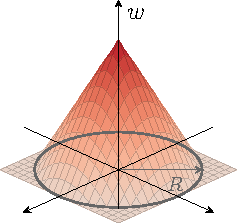
\includegraphics{figures/03_comparison_TO_TTO/01_circ_filter/filt_cir.pdf}
    \caption{Kernel of the 2D convolution operator.}
    \label{fig:03_ker}
\end{marginfigure} 
The filtered values of the design variable calculated as:
\begin{equation}
    \rhofil_i = \frac{\sum_{j \in \mathbb{N}_{i,R}} w(d_j)v_j\rho_j}{\sum_{j \in \mathbb{N}_{i,R}} w(d_j)v_j}.
    \label{eq:03_rhofil}
\end{equation}
As the filtering phase produces a large quantity of gray elements, a smooth projection technique based on the \textit{tanh} function is implemented~\sidecite{wang_projection_2011}:
\begin{equation}
    \rhophys_j = \frac{\tanh(\beta\eta)+\tanh(\beta(\rhofil_j - \eta))}{\tanh(\beta\eta)+\tanh(\beta(1 - \eta))},
    \label{eq:03_proj}
\end{equation}
where $\beta$ is a parameter that define the slope of this approximation function: the larger the value of $\beta$, the less intermediate elements are present in the structure topology. $\eta$ is the threshold value of the projection. Using \eqref{eq:03_proj} is not volume conservative for all values of $\eta$, and to stay conservative we use a volume-increasing filter~\sidecite{ferrari_new_2020}. The value of $\eta = 0.4$ is then chosen.

The derivative of the filtered density $\vect{\rhofil}$ with respect to the design variable $\vect{\rho}$ is written deriving \eqref{eq:03_rhofil}:
\begin{equation}
    \derfrac{\rhofil_i}{\rho_j} = \frac{w(d_j)v_j}{\sum_{j \in \mathbb{N}_{i,R}} w(d_j)v_j}.
    \label{eq:03_sens_filt}
\end{equation}
The sensitivity of the physical densities $\bm{\rhophys}$ with respect to the filtered $\bm{\rhofil}$ can be written as:
\begin{equation}
    \derfrac{\rhophys_j}{\rhofil_j} = \beta \frac{1-\tanh^2(\beta(\rhofil_j-\eta))}{\tanh(\beta\eta)+\tanh(\beta(1 - \eta))}.
    \label{eq:03_sens_proj}
\end{equation}
Using the chain rule it is possible to write:
\begin{equation}
    \label{eq:03_chain}
    \derfrac{h}{\rho_i} = \sum_{j \in \mathbb{N}_{i,R}} \derfrac{f}{\rhophys_j} \derfrac{\rhophys_j}{\rhofil_j} \derfrac{\rhofil_j}{\rho_i},
\end{equation}
where $h$ represents a generic function.
\paragraph{Objective and constraint funtions}
Up until this point, we have been focused on the compliance minimization formulation \eqrefnotext{eq:03_prob-comp}. Moving forward, we introduce the necessary modifications to transition into the volume minimization formulation with stress constraints. This formulation will be used to compare the continuous mesh with truss-link structure optimization.

The objective of the optimization is to minimize the volume of a structure subject to a specified load case. The volume of the structure $V$ is expressed in percentage with respect to the total volume $V_0$ of the domain $\Omega$:
\begin{equation}
    V = \frac{1}{V_0}\sum_{i \in \Omega} \rhophys_i v_i,
    \label{eq:03_vol_v}
\end{equation}
where $v_i$ is the elementary volume occupied by the $i$-th element. In this thesis, we assume that $v_i$ is equal for all the elements, and thus \eqref{eq:03_vol_v} is simplified as follows:
\begin{equation}
    V = \frac{1}{N_{e}} \sum_{i \in \Omega} \rhophys_i. 
    \label{eq:03_obj_vol}  
\end{equation}

The normalized local stress constraint $\vect{g}_{\text{st}}$ are formulated as:
\begin{equation}
    \frac{\sigma_{\text{VM},j}}{\sigma_L}-1 \leq 0, \quad \forall j \in \Omega_{mat}(\bm{\rho})
    \tag{$g_{\text{st}}$}
\end{equation}
where $\Omega_{mat}(\bm{\rho}) \subseteq \Omega$ represents the design-dependent set of elements with a non-zero density, $\sigma_{\text{VM},j}$ is the equivalent von Mises stress for the $j$-th element, and $\sigma_L$ is the maximum allowable of the material.

A first difficulty that arises is that the stress constraints are defined only for the elements where $\rhophys_i > 0$, while $\rhophys_i\in[0,1]$. Thus, the set of constraints changes during the optimization. This class of problems are called \acrfull{mpvc}~\sidecite{achtziger_mathematical_2008} and are known for being difficult to solve with a gradient descent optimization algorithm. The original set of constraints $\vect{g}_{\text{st}}$ is then reformulated into an equivalent design-independent set of constraints $\bar{\vect{g}}_{\text{st}}$ as follows~\sidecite{cheng_study_1992}:
\begin{equation}
    \rhophys_i\left(\frac{ \sigma_{\text{VM},i}}{\sigma_L}-1 \right) \leq 0, \quad \forall i \in \Omega.
    \tag{$\bar{g}_{\text{st}}$}
\end{equation}

\paragraph{Von Mises stress evaluation}
The evaluation of the equivalent stress of an element follows the formulation proposed by Von Mises. Let us take a four-nodes quadrilateral linear element with a single integration (or Gauss) point in the center and four $2a$ equal-length sides (see \figref{fig:03_gp}). If bilinear shape function are used to interpolate the displacement field, we can evaluate the deformations at the integration point as:
\begin{equation}
    \begin{pmatrix}
    \varepsilon_x \\
    \varepsilon_y \\
    \gamma_{xy}
    \end{pmatrix} = \matr{B}_s\vect{q}_s
    \textrm{,  with }
    \matr{B}_s =
    \frac{1}{4a}
    \begin{pmatrix}
    -1  &   1   &   1   &   -1  &   0   &   0   &   0   &   0   \\
    0   &   0   &   0   &   0   &   -1  &   -1  &   1   &   1   \\
    -1  &   -1  &   1   &   1   &   -1  &   1   &   1   &   -1
    \end{pmatrix},
\end{equation}
where $\vect{q}_s = (u_1, u_2, u_3, u_4, v_1, v_2, v_3, v_4)^T$ represents the vector of the displacement degrees of freedom of the element. 

\begin{marginfigure}
    \centering
    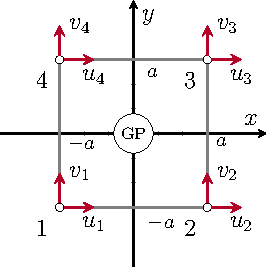
\includegraphics{figures/03_comparison_TO_TTO/02_gauss_point/gp.pdf}
    \caption{A four-node quadrilateral element. GP is the Gaussian integration point for which the equivalent stress is evaluated.}
    \label{fig:03_gp}
\end{marginfigure}


The stress tensor is evaluated using the elasticity Hooke's law in 2D as follows: 
\begin{equation}
    \begin{pmatrix}
    \sigma_x \\
    \sigma_y \\
    \tau_{xy}
    \end{pmatrix}
    =\matr{C}_e
    \begin{pmatrix}
    \varepsilon_x \\
    \varepsilon_y \\
    \gamma_{xy}
%     \end{pmatrix},
%     \quad
%    \text{with }
    \end{pmatrix}
    \quad
    \text{with}
    \quad
    \matr{C}_e = \frac{E}{1-\nu^2}
    \begin{pmatrix}
    1   &   \nu &   0   \\
    \nu &   1   &   0   \\
    0   &   0   &   G
    \end{pmatrix}.
\end{equation}

The equivalent Von Mises stress of the element can then be written as:
\begin{align}
    \langle \vect{\sigma}_{\text{VM}} \rangle &= \sqrt{\sigma_x^2 + \sigma_y^2 - \sigma_x \sigma_y+3\tau_{xy}} \\
    &= \sqrt{
    \begin{pmatrix}
    \sigma_x & \sigma_y & \tau_{xy}
    \end{pmatrix}
    \begin{pmatrix}
    1       &   -1/2    &   0   \\
    -1/2    &   1       &   0   \\
    0       &   0       &   3
    \end{pmatrix}
    \begin{pmatrix}
    \sigma_x \\
    \sigma_y \\
    \tau_{xy}
    \end{pmatrix}} \\
    &= \sqrt{\vect{q}_s^T\matr{B}_s^T\matr{C}_e^T\matr{D}_{\text{VM}}\matr{C}_e\matr{B}_s\vect{q}_s}
    \textrm{,  with } \matr{D}_{\text{VM}} = 
    \begin{pmatrix}
    1       &   -1/2    &   0   \\
    -1/2    &   1       &   0   \\
    0       &   0       &   3
    \end{pmatrix} \\
    \langle \vect{\sigma}_{\text{VM}} \rangle &= \sqrt{\vect{q}_s^T\matr{S}\vect{q}_s}, \quad
    \textrm{with } \matr{S} = \matr{B}_s^T\matr{C}_e^T\matr{D}_{\text{VM}}\matr{C}_e\matr{B}_s
    \label{eq:03_VM_calc}
\end{align}

\paragraph{Microscopic and macroscopic stress}
In stress-constrained topology optimization the element stress is usually evaluated using the microscopic stress formulation, assuming that there is no direct correlation between stress and density~\sidecite{duysinx_topology_1998}. Indeed, the use of the macroscopic stress in volume minimization optimization problems creates all-void design~\sidecite{le_stress-based_2010}. The properties that the microscopic stress should present are:
\begin{enumerate}[label=(\roman*)]
    \item The stress criterion should be mathematically as simple as possible, as the relationship between Young's modulus and density. This permits a simple numerical implementation.
    \item To mimic the real physical behavior, the microscopic stress should be inversely proportional to density.
    \item The microscopic stress should converge to a non-zero value at zero density. This requisite is deduced from investigations into the asymptotic stress behavior in thin layers~\sidecite{verbart_unified_2017}.
\end{enumerate}

The relation within stress and displacement is written as:
\begin{equation}
    \langle \vect{\sigma}_{\text{VM}} \rangle = \matr{C}_e(\langle E \rangle) \langle \vect{\varepsilon} \rangle
    \label{eq:03_stress_disp}
\end{equation}
where the variables between angular brackets $\langle \dots \rangle$ represent macroscopic variables.

Combining (i) and (ii) with \eqsref{eq:03_simp} and \eqrefnotext{eq:03_stress_disp}, the microscopic stress can be written as:
\begin{equation}
    \vect{\sigma}_{\text{VM}} = \frac{\langle \vect{\sigma}_{\text{VM}} \rangle}{\rho^q_e} = \rho_e^{p-q} \matr{C}_e(E_0)\langle \vect{\varepsilon} \rangle
\end{equation}
where the exponent $q$ is a number greater than 1.

One possible choice that satisfy all the requirements is $q=p$~\sidecite{le_stress-based_2010,verbart_unified_2017,holmberg_stress_2013,da_silva_stress-constrained_2019}. Thus, the microscopic stress is defined as:
\begin{equation}
    \vect{\sigma}_{\text{VM}} = \matr{C}_e(E_0)\langle \vect{\varepsilon} \rangle
    \label{eq:03_micro_stress}
\end{equation}
From a physical perspective, the significance of microscopic stress becomes evident when considering an element with intermediate density and a porous microstructure. The microscopic stress presented in \eqref{eq:03_micro_stress} measures the stress of the microstructure. It is grounded in the assumption that the macroscopic deformations of the homogenized element generate within the microstructure of the element a stress state that remains unaffected by the density of the element itself.

\paragraph{Constraints aggregation and relaxation}
When optimizing a structure with stress constraints using a \gls{nand} formulation, two primary challenges commonly arise:
\begin{enumerate}[label=(\roman*)]
    \item Is it known in the literature \cite{rozvany_design-dependent_2001,stolpe_models_2003} that stress-based topolgy optimization suffer from the \textit{singular minima} (or \textit{singularity}) problem: firstly observed on truss structure optimization \cite{sved_structural_1968}, these \textit{minima} are almost inaccessible to standard gradient-based optimizer, and they represent the \textit{minima} of the optimization. This because achieving the optimal solution to a problem using continuous design variables may necessitate passing through a state where the optimization constraints are violated, \ie the \textit{minimum} is on a lower dimension compared to the design space. This problem is often solved using a technique called \textit{constraints relaxation}~\sidecite{cheng_relaxed_1997}.

    \item The stress is a local measure, and thus a large set of constraints is generated when a reasonably fine mesh is used (one element, one constraint). This problem is often solved using a technique called \textit{constraints aggregation} or \textit{global constraints}~\sidecite{da_silva_local_2021}.
\end{enumerate} 

Following the work developed by Verbart \etal~\sideciteonce{verbart_unified_2017}, the lower bound \gls{ks} function~\sidecite{kreisselmeier_systematic_1979} is used to approximate the local relaxed stress constraint maximum. The authors discovered that employing lower-bound \gls{ks} aggregation functions to approximate the maximum operator in stress-constrained topology optimization eliminates the need for stress constraint relaxation methods to address the singularity issue. This is because the lower-bound functions inherently offer a combined effect of constraints aggregation and relaxation. The \gls{ks} aggregated stress constraint function is defined as follows:
\begin{equation} 
    G_{\text{KS}}^\text{L} = \frac{1}{P} \ln{\left( \frac{1}{N_e} \sum e^{{P}\bar{g}_i} \right)}.
    \label{eq:03_gksl}
\end{equation}
Its main advantage over other different formulations is that it uses a single hyperparameter $P$ to control the aggregation and the relaxation of the constraints simultaneously.

\paragraph{Minimum volume formulation}
The \gls{nand} minimum volume formulation for continuous discretization is written \eqsref{eq:03_obj_vol} and \eqrefnotext{eq:03_gksl} as:
\begin{equation}
    \begin{aligned}
    \min_{\bm{\rho}}         && V &= \frac{1}{N_{e}} \sum_{i \in \Omega} \rhophys_i,  \\
    \textrm{s.t.}   && G_{\text{KS}}^\text{L} &= \frac{1}{P} \ln{\left( \frac{1}{N_e} \sum_{i \in \Omega} e^{{P}\bar{g}_i} \right)} \leq 0 \\
    && \bm{K}\bm{u} &= \bm{F}\\
    && 0 &\leq \rho_i \leq 1, \\
    \end{aligned}
    \tag{$\mathbb{T}_1$}
    \label{eq:03_prob-stress}
\end{equation}
The optimization is carried out using a gradient descent optimization algorithm for which the sensitivities are given in analytical form. Using analytic gradients is in general more efficient than finite differences as it avoids the need for multiple function evaluations, making the optimization process faster and more precise.

\paragraph{Sensitivity analysis of the objective function}
The objective of this section is to quickly present the calculation of the analytical sensitivity of the volume with respect to the design variable $\rho$. Deriving \eqref{eq:03_obj_vol} we obtain:

\begin{equation}
    \derfrac{V}{\rhophys_i} = \frac{1}{N_{e}}.
    \label{eq:03_01}
\end{equation}
The sensitivity of the objective function can then be evaluated using \eqsref{eq:03_01} \eqrefnotext{eq:03_sens_filt}, \eqrefnotext{eq:03_sens_proj}, and \eqrefnotext{eq:03_chain} as follows:
\begin{equation}
    \frac{d V}{d \rho_i} = \sum_{j \in \mathbb{N}_{i,R}} \derfrac{V}{\rhophys_j} \derfrac{\rhophys_j}{\rhofil_j} \derfrac{\rhofil_j}{\rho_i}.
\end{equation}
\paragraph{Sensitivity analysis of the constraint function}
This section focuses on the details of the calculation of how the constraint function $G_{\text{KS}}^\text{L}$ changes with respect to the design variable $\vect{\rho}$.

As the constraint function $G_{\text{KS}}^\text{L} = G(\vect{\rhophys}, \vect{u}(\vect{\rhophys}) )$ is explicitly and implicitly (via the relationship with $\vect{u}$) depending on $\vect{\rhophys}$, the first-order derivative is evaluated using the total derivative formula:
\begin{equation} \label{eq:sens-0}
    \derfrac{G_{\text{KS}}^\text{L}}{\rhophys_j} = \frac{d G}{d \rhophys_j} = \derfrac{G}{ \rhophys_j} + \derfrac{G}{\vect{u}} \frac{d \vect{u} }{d \rhophys_j}
\end{equation}
As function $G_{\text{KS}}^\text{L}$ depends on $\vect{u}$ via the stresses $\sigma_i$, it is possible to write:
\begin{equation} \label{eq:sens-1}
    \derfrac{G}{\vect{u}} = \sum_{i \in \Omega} \left( \derfrac{G}{\sigma_i} \derfrac{\sigma_i}{\vect{u}}\right)
\end{equation}
Combining Eq. \ref{eq:sens-0} with Eq. \ref{eq:sens-1}, we obtain:
\begin{equation} \label{eq:sens-2}
    \frac{d G}{d \rhophys_j} = \underbrace{\derfrac{G}{\rhophys_j}}_A + \sum_{i \in \Omega} \left( \underbrace{\derfrac{G}{\sigma_i}}_B \underbrace{\derfrac{\sigma_i}{\vect{u}}}_C \right)  \underbrace{\frac{d \vect{u} }{d \rhophys_j}}_D
\end{equation}
We compute the four factors separately:
\begin{enumerate}[label=\Alph* --]
    \item The first term represents the explicit relationship of $G$ to the physical densities and its calculation is straightforward: 

    \begin{equation} \label{eq:sens-2-1}
        \derfrac{G}{ \rhophys_j} = \frac{1}{P} \frac{\left(\frac{ \sigma_{\text{VM},j}}{\sigma_L}-1 \right)\frac{1}{N_e} P e^{{P}\bar{g}_j}}{\frac{1}{N_e} \sum_k e^{{P}\bar{g}_k}} = \left(\frac{ \sigma_{\text{VM},j}}{\sigma_L}-1 \right) \frac{e^{{P}\bar{g}_j}}{\sum_k e^{{P}\bar{g}_k}}
    \end{equation}
    
    \item The second term can be calculated using the chain rule:
    \begin{equation}
        \label{eq:sens-2-2}
        \derfrac{G}{\sigma_i} = \derfrac{G}{\bar{g}_i} \derfrac{\bar{g}_i}{\sigma_i} = \frac{1}{P} \frac{\frac{1}{N_e} P e^{{P}\bar{g}_i}}{\frac{1}{N_e} \sum_k e^{{P}\bar{g}_k}} \frac{\rhophys_i}{\sigma_L} = \frac{\rhophys_i}{\sigma_L} \frac{e^{{P}\bar{g}_i}}{\sum_k e^{{P}\bar{g}_k}}
    \end{equation}
    
    \item We reformulate Eq. \ref{eq:03_VM_calc} to be written in global coordinates instead of local:
    \begin{equation}
        \label{eq:sens-3}
        \sigma_i^2 = \vect{q}_s^T\matr{S}\vect{q}_s = \vect{u}^T |\matr{S_i}|_g \vect{u}
    \end{equation}  
    where $|\matr{S_i}|_g$ represents the matrix $\matr{S}$ of \eqref{eq:03_VM_calc}written on global coordinates \sidenote{The matrix $|\matr{S_i}|_g$ can be calculated using the very same assmebling approach used for the stiffness matrix $\matr{K}$ starting from the elemental stiffness matrix $\matr{K}_e$. As the global stiffness matrix $\matr{K}$, $|\matr{S_i}|_g$ is symmetric and sparse.}. We can now differentiate \eqref{eq:sens-3} with respect of the displacement field in global coordinates $\vect{u}$ to obtain:
    \begin{equation}
        \label{eq:sens-4}
        \derfrac{\sigma_i}{\vect{u}} = \frac{|\matr{S_i}|_g \vect{u}}{\sigma_i}
    \end{equation}
    \eqsref{eq:sens-2-2} and \eqrefnotext{eq:sens-4} are now combined to obtain the result of the product of the \textbf{B} and \textbf{C} terms. As a result, the derivatives of $G$ with respect to $\bm{u}$, are written as:
    \begin{equation} \label{eq:sens-4-1}
        \derfrac{G}{\vect{u}} = \frac{\frac{\rhophys_j}{\sigma_L\sigma_j} e^{{P}\bar{g}_i}}{\sum_i e^{{P}\bar{g}_i}} |\bm{S_j}|_g \bm{u}
    \end{equation}

    \item To calculate the last term, we take the static equilibrium equation $\matr{K}\vect{u} = \vect{f}$ and differentiating it with respect to the physical densities $\rhophys_j$, obtaining:
    \begin{equation}
        \derfrac{\matr{K}}{\rhophys_j}\vect{u} + \matr{K}\derfrac{\vect{u}}{\rhophys_j} = 0 \iff \derfrac{\vect{u}}{\rhophys_j} = -\matr{K}^{-1}\derfrac{\matr{K}}{\rhophys_j}\vect{u},
    \end{equation}
    where
    \begin{equation}
        \label{eq:sens-5}
        \derfrac{\matr{K}}{\rhophys_{j}} = (E_0-E_{\textrm{min}}) p\rhophys_j^{p-1} \matr{K}_{e,j}.
    \end{equation}
    \eqref{eq:sens-5} represent the well known first-derivative term of the global stiffness matrix $\matr{K}$ with respect of the physical densities $\rhophys_j$ when using \gls{simp} material scheme~\sidecite{bendsoe_topology_2004}. We finally obtain the last term:
    \begin{equation} \label{eq:sens-6}
        \frac{d \vect{u} }{d \rhophys_j} = - \matr{K}^{-1} \left((E_0-E_{\textrm{min}}) p\rhophys_j^{p-1} \matr{K}_e \right) \vect{u}
    \end{equation}
\end{enumerate}

Combining Eq. \ref{eq:sens-2}, Eq. \ref{eq:sens-2-1}, Eq. \ref{eq:sens-4-1}, and Eq. \ref{eq:sens-6}, we finally obtain:
\begin{equation}
\derfrac{G_{\text{KS}}^\text{L}}{\rhophys_j} = \left(\frac{ \sigma_{\text{VM},j}}{\sigma_L}-1 \right) \frac{e^{{P}\bar{g}_j}}{\sum_k e^{{P}\bar{g}_k}} - 
\matr{K}^{-1}\derfrac{G}{\vect{u}} \left(\derfrac{\matr{K}}{\rhophys_{j}} \right) \vect{u}
\end{equation}

To avoid the explicit calculation of $\matr{K}^{-1}$ we use the \textit{adjoint method}\sidenote{More information about the adjoint method used to analytically calculate the first-order derivatives can be found on the Martins \etal book \cite{martins_engineering_2021}.}. Here is the linear system that, once solved, permits to calculate $\vect{\psi}$:
\begin{equation} \label{eq:sens-98}
    \matr{K}\vect{\psi} = \derfrac{G}{\vect{u}} \iff \vect{\psi} = \matr{K}^{-1}\derfrac{G}{\vect{u}}
\end{equation}
This formula is called \textit{adjoint equation}. This equation is solved for $\vect{\psi}$ and the result used to evaluate:
\begin{equation}\label{eq:sens-99}
\derfrac{G_{\text{KS}}^\text{L}}{\rhophys_j} = \left(\frac{ \sigma_{\text{VM},j}}{\sigma_L}-1 \right) \frac{e^{{P}\bar{g}_j}}{\sum_k e^{{P}\bar{g}_k}} - \vect{\psi} \left(\derfrac{\matr{K}}{\rhophys_{j}}\right) \vect{u}
\end{equation}
\marginnote{Solving linear system \ref{eq:sens-98} instead of directly calculating the inverse matrix of $\matr{K}$ is more efficient from a performance perspective. The cost of solving a system using the Cholesky decomposition is $\mathcal{O}(N^3/3)$, while a matrix inversion is $\mathcal{O}(N^3)$.} where $N$ represents the size of the square matrix describing the linear system.
\eqref{eq:sens-99} represents the first-order derivative equation used to evaluate the sensitivity of the constraint function $G_{\text{KS}}^\text{L}$ with respect to the physical densities $\vect{\rhophys}$. The value of $\vect{\psi}$ is calculated every iteration solving the linear system \ref{eq:sens-98}.

The sensitivity of the aggregated contraint function with respect to the design variable $\vect{\rho}$ is evaluated using \eqsref{eq:03_01} \eqrefnotext{eq:03_sens_filt}, \eqrefnotext{eq:03_sens_proj}, and \eqrefnotext{eq:03_chain} as follows:
\begin{equation}
    \frac{d G_{\text{KS}}^\text{L}}{d \rho_i} = \sum_{j \in \mathbb{N}_{i,R}} \derfrac{G_{\text{KS}}^\text{L}}{\rhophys_j} \derfrac{\rhophys_j}{\rhofil_j} \derfrac{\rhofil_j}{\rho_i}.
\end{equation}

\subsection{Truss discretization \gls{sand} minimum volume formulation}
We are now shifting our focus from continuous structures to discrete truss systems, describing the \gls{tto} (also knows in early literature as layout optimization), a structure optimization method that focuses on discrete structures. In his most used formulation, \gls{tto} aims at reducing material usage while meeting stress criteria using a \gls{sand} approach. The problem is already well-posed for the comparison with continuous discretization, and our intention is to now explore specific key concepts within its established framework.
\paragraph{Classical Michell structures} \label{sec:03_michell}
The characteristics of these structures are described by some simple criteria that date to the end of the 19th and the beginning of the 20th century. When a structure is statically determinate — \ie the structure is not a mechanism, and it is not over-constrained by the supports — the Maxwell theorem~\sidecite{maxwell_ireciprocal_1870} states that:
\begin{equation} \label{eq:maxwell-th}
    \sum_{\forall i | q_i>0}\ell_iq_i + \sum_{\forall i | q_i<0}\ell_iq_i = \textrm{const.}
\end{equation}
where $\ell_i$ and $q_i$ represent the length and the axial force of the $i$-th member, respectively. The constant value at the right of~\eqref{eq:maxwell-th} depends on the nature of the boundary conditions and the material used. The Maxwell theorem dictates that any increment in compression forces must be counterbalanced by an equivalent increase in tension forces when the structure remains topologically unchanged. So for statically determinate structures the structure layout is not influenced by the ratio between $\sigma_\text{c}$ and $\sigma_\text{t}$, the Young's modulus $E$ of the material, nor the force magnitude.

Starting from Maxwell's findings, Michell theorized two further criteria for optimal truss structures~\sidecite{michell_limits_1904} valid when the maximum allowable stress is equal in tension and compression ($\sigma_\text{t} = \sigma_\text{c}$) and when the supports of the structure are statically determinate. The first one states that all the members of an optimal structure should present internal stress equal in magnitude to the maximum allowable value of the material - \ie the structure is \textit{fully stressed}. The second criterion asserts that the strain of all the members of the structure should be equal and there should be no other point having a strain higher than this value. As formulated, these two criteria are known as the Michell criteria. The second criterion was later generalized by Hemp~\sidecite{hemp_optimum_1973} as:
\begin{equation} \label{eq:hemp}
    -\frac{1}{\sigma_\text{c}}\leq \varepsilon \leq \frac{1}{\sigma_\text{t}}
\end{equation}
Compared to the second Michell criterion, \eqref{eq:hemp} permits to correctly identify the minimum volume structure even when different strength values for compression and tension and different support types are taken. These criteria are known as the Michell-Hemp criteria.

\paragraph{Plastic material formulation}
The rigid-plastic formulation characterizes the material as entirely rigid up to the point of reaching the yield stress, denoted as $\sigma_y$, and subsequently assumes a constant stress level of $\sigma_y$ once that threshold is exceeded. This formulation is a clear consequence of the application of the Michell-Hemp criteria and has thus been used in the very first work of layout optimization (also known as \gls{tto})~\sidecite{dorn_automatic_1964,chan_optimum_1964,hemp_optimum_1973}. 

\paragraph{The ground structure approach}
The ground structure is a framework composed of various structural members that connect specified points or nodes in two- or three-dimensional space (see \figref{fig:03_mesh_d}). These members can take the form of beams, columns, wires, or bars elements, depending on the specific structural requirements. In this thesis we will deal with trusses, and so the chosen element is the bar. Since the nodes within the ground structure are considered pin-joints, all straight members exclusively face either tension or compression loads. 
\begin{marginfigure}
    \centering
    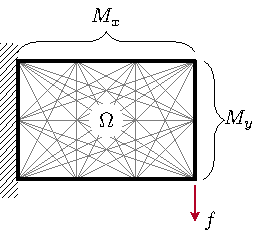
\includegraphics{figures/03_comparison_TO_TTO/03_disc_mesh/d_mesh.pdf}
    \caption{The domain $\Omega$ is discretized using a set of straight members connecting a set of nodes. THis framework is known as ground structure.}
    \label{fig:03_mesh_d}
\end{marginfigure}

Depending on how the connectivity of the grid of nodes is, we can experience very different ground structures. In a fully connected ground structure, every node within the system is linked to every other node, resulting in a dense and redundant structural configuration. The number of bars $N_{\text{el}}$ of a fully connected ground structure can be determined using the following formula:
\begin{equation}
    N_{\text{el}} = \frac{M \cdot (M-1)}{2}
\end{equation}
where $M$ represent the number of nodes of the structure.

In classic works, the ground structure is used as the start of the optimization, where the optimized structure is obtained as a subset of the initial ground structure, but multiple alternative approaches have been proposed since then, \eg starting from a very coarse ground structure that is enriched during the analysis~\sidecite{gilbert_layout_2003}, or giving the nodes of a coarse ground structure the possibility to move, during~\sidecite{pedersen_optimal_1973, achtziger_simultaneous_2007, descamps_lower-bound_2013}, or after the optimization, simultaneously reducing the number of active members of the solution~\sidecite{he_rationalization_2015, lu_reducing_2023}.

\paragraph{Optimization formulation}
The volume minimization formulation with maximum stress constraints is stated in terms of members' cross-sectional areas $\vect{a}$ and member forces $\vect{q}$ as follows:
\begin{equation}
    \begin{aligned}
    \min_{\vect{a}, \vect{q}}   && V &= \vect{\ell}^{T}\vect{a} && \textrm{(Volume)}\\
    \textrm{s.t.}   && \matr{B}_s\vect{q} &= \vect{f} && \textrm{(Force equilibrium)}\\
    && -\sigma_\text{c}\vect{a} &\leq \vect{q} \leq \sigma_\text{t}\vect{a} && \textrm{(Stress constraints)} \\
    && \vect{a} &\geq 0, \\
    \end{aligned}
    \tag{$\mathbb{P}_0$}
    \label{eq:03_optim_original}
\end{equation}
where $\matr{B}_s$ is a $N_{\text{dof}} \times N_{\text{el}}$ matrix containing the direction cosines of the $j$-th member with respect to the $i$-th degree of freedom to calculate the nodal force equilibrium, and where $N_{\text{dof}}$ is the number of \gls{dofs}, equal to $2M$ or $3M$ for a two- or a three-dimensional load case, respectively. $\vect{q} = [q_1, q_2, \ldots,q_{N_{\text{el}}}]^T$ is the vector containing the internal member forces, with a positive sign when in tension, caused by the external load $\vect{f} = [f_1, f_2, \ldots,f_{N_{\text{dof}}}]^T$. The state variable $\vect{a} = [a_1, a_2, \ldots,a_{N_{\text{el}}}]^T$ represents the cross-sectional area of the $N_{\text{el}}$ members of the structure. $\sigma_\text{c}$ and $\sigma_\text{t}$ are the compressive and tensile maximum allowable stresses of the material, respectively. This formulation takes into account only the linear behavior of the structure and is equivalent to the original and well-studied member force formulation~\sidecite{dorn_automatic_1964, bendsoe_topology_2004}.

The resolution of Problem \ref{eq:03_optim_original} frequently produces complex structures made up of a multitude of small members that tends to the shapes of Michell structures (see Fig~\ref{fig:truss-ex})~\sidecite{michell_limits_1904,gilbert_layout_2003}. While it is known that these structures are nearly optimal, one would want to limit the complexity of the resulting structure. Substituting $\vect{\ell}$ with $\vect{\tilde{\ell}} = [\ell_1 + s, \ell_2 + s, \ldots,\ell_{N\text{el}} + s]^T$ in the objective function of \ref{eq:03_optim_original}, one would penalize the appearance of small members~\sidecite{parkes_joints_1975}. $\vect{\tilde{\ell}}$ is called augmented member length and $s$ the joint cost. This approach mimics the mesh-independency regularization filter of topology optimization, avoiding the inevitable apparition of structures with tiny features when a fine mesh is adopted.

\begin{marginfigure}
    \centering
    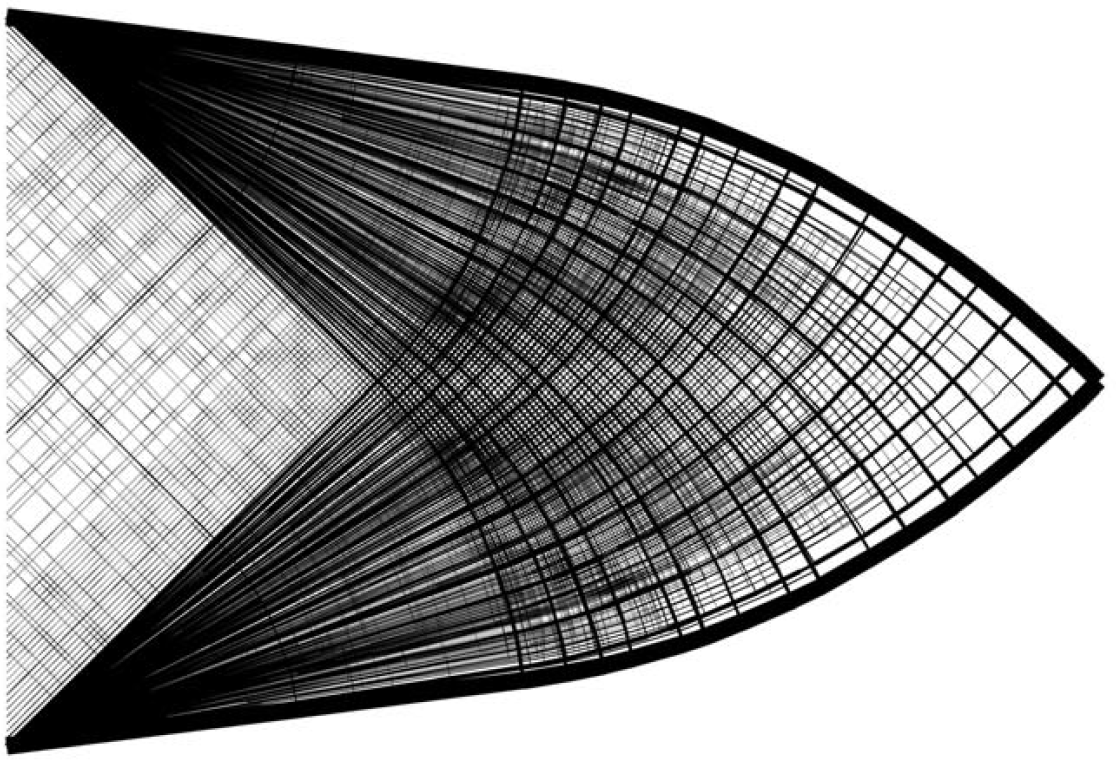
\includegraphics[width=\linewidth]{figures/03_comparison_TO_TTO/truss-ex.png}
    \caption{The optimal structures found by layout optimization tend at Michell-like structures, made up by a very large number of infinitesimal struts \cite{gilbert_layout_2003}.}
    \label{fig:truss-ex}
\end{marginfigure}

\section{Comparison between continuous and truss discretization} \label{sec:03_comparison}
In the upcoming discussion, we will be comparing the optimized structures using discrete and continuous meshes. Our primary objective in this comparison is to gain a comprehensive understanding of the application limits inherent in these two structural discretization methods. If, indeed, we identify such limitations, the aim is to discern and define them. 

Since our interest in ultralight structures, we are especially interested in comparing the results of both optimization methods when dealing with different volume fractions on a common load case. Since we can't directly control volume in our formulation, we will adjust the material properties to influence the volume fraction of the optimized structure. For this comparative analysis, we have selected three key performance metrics: the volume fraction $V_\text{f}=V/\Omega$, the structural compliance $C$, and the maximum material allowable $\sigma_L$. Among these, we classify stress limit as the active metric used to influence the optimization, while volume and compliance are the objective of the optimization and a passive metric, respectively. In addition to the aforementioned performance metrics, we will also track the execution time of the algorithms.

\subsection{Definition of a common test case}
\begin{figure}[]
    \centering
    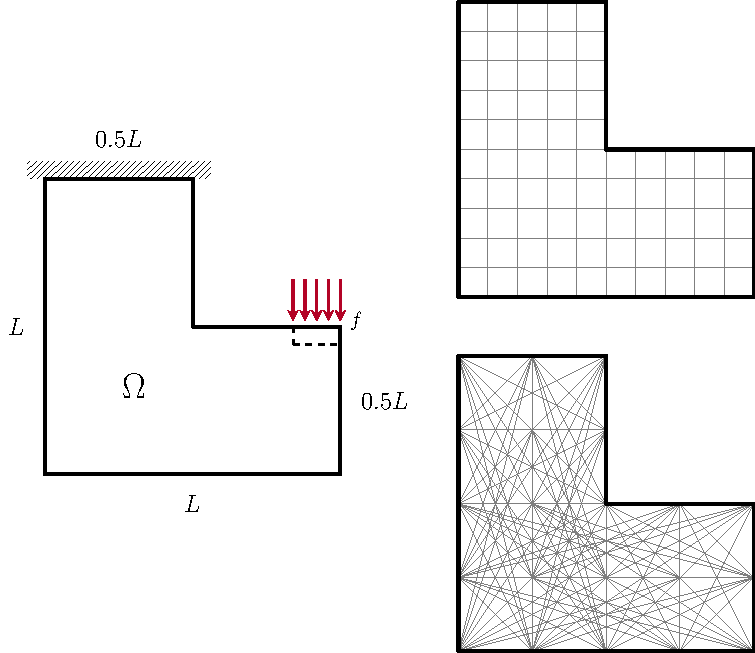
\includegraphics[scale=0.75]{figures/03_comparison_TO_TTO/04_L_bc/L_bc.pdf}
    \caption{\todo{caption}}
    \label{fig:03_L_bc}
\end{figure}
The L-shape beam is one of the most used load case benchmark for stress based topology optimization~\sidecite{duysinx_topology_1998,le_stress-based_2010}. This choice is driven by the distinctive geometry of the problem, which generates a stress concentration, particularly at the sharp corner—a phenomenon approaching infinity. Consequently, optimized solutions often feature a large fillet, mitigating the intensity of the stress singularity. The geometric description of the test case is given in \figref{fig:03_L_bc}. The beam with dimensions $L\times L$ present an encastre on the top part and a load on the rigth extremity. For the continuous mesh case the load is distributed over multiple elements (5\% of $L$) to avoid stress concentrations and the stress constraints are not evalued there. This zone is considered outside of the design domain $\Omega$.

To permit the discretization comparison, the structure is divided into two distinct meshes: in the continuous case, we employ a mesh consisting of $600\times600$ quadrilateral elements, totaling \num[group-separator={$\,$}]{270000} elements, while for the truss configuration, we employ a mesh with $33\times 33$ nodes and a fully connected ground structure, comprising a total of \num[group-separator={$\,$}]{305728} candidates.

We employ the same isotropic material and structure dimensions for the two optimization, and the complete data is resumed in \tabref{tab:03_mat}. The value of the maximum material admissible $\sigma_\text{L}$ is used as the parameter that influences the volume fraction of the solutions. For simplicity, all numeric values are assumed normalized and dimensionless.

\begin{margintable}[]
    \centering
    \begin{tabular}{cc}
    \toprule
    \textbf{Parameter}        & \textbf{Value} \\ \midrule
    $E$              & 1     \\
    $\nu$            & 0.3   \\
    $L$              & 100   \\
    $\sigma_\text{L}$ & var. \\
    \bottomrule
    \end{tabular}
    \caption{Material data used for the optimizations. The value of the maximum material admissible $\sigma_\text{L}$ is used as the parameter to generate multiple optimized topologies.}
    \label{tab:03_mat}
\end{margintable}

\subsection{Numerical application}
The focus of this section is to provide the numerical framework used to carry out the comparative analysis of the optimization results obtained from continuous and truss discretizations. The optimization formulations previously described have been implemented using Python.

The optimizing algorithm chosen for the continuous mesh is the \gls{mma}~\sidecite{svanberg_method_1987}. The parameter called \textit{movelimit}\sidenote{More information on the implementation of the \textit{movelimit} parameter can be found on the paper by Verbart \cite{verbart_unified_2017}} is set to $0.1$ while the other algorithm's parameters are set to their default value. A continuation scheme for the aggressiveness of the projection parameter $\beta$ is set to increase by one every 200 iterations, the number of max iteration is set to 7500, the stopping criteria is calculated as $\Vert r_k \Vert_2 / \sqrt{N_e}$ on the physical densities $\rhophys$ \cite{ferrari_new_2020}, and it is set to $10^{-4}$. The aggregation parameter $P$ of the aggregation function $G_{\text{KS}}^\text{L}$ is set to 32. The numerical implementation is carried out using the NLopt Python optimization framework~\sidecite{NLopt_2007}, using the \todo{sensitivity}.

Formulation \ref{eq:03_optim_original} represents a \gls{lp} problem that can be efficiently solved by modern algorithms. In this work, we used the Python package CVXPY 1.2.2~\sidecite{diamond_cvxpy_2016} with the ECOS 2.0.7~\sidecite{domahidi_ecos_2013} solver. As Formulation is linear, no sensitivity calculation is carried out.

The optimizations presented in this section are performed on a server
equipped with an Intel® Core™ \todo{totot}
and 6 GB of RAM.

\paragraph{Coninuous mesh optimization results}
\begin{figure*}[]
    \subcaptionbox{}{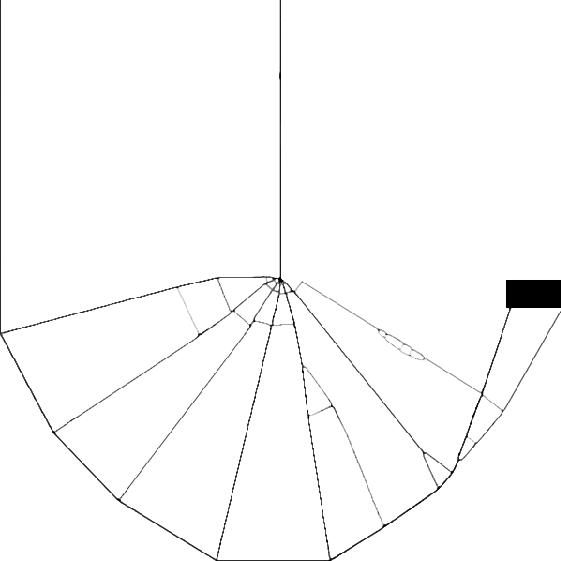
\includegraphics[width=0.23\linewidth ]{figures/03_comparison_TO_TTO/05_to_sol/fig0_10.pdf}}
    \hfill
    \subcaptionbox{}{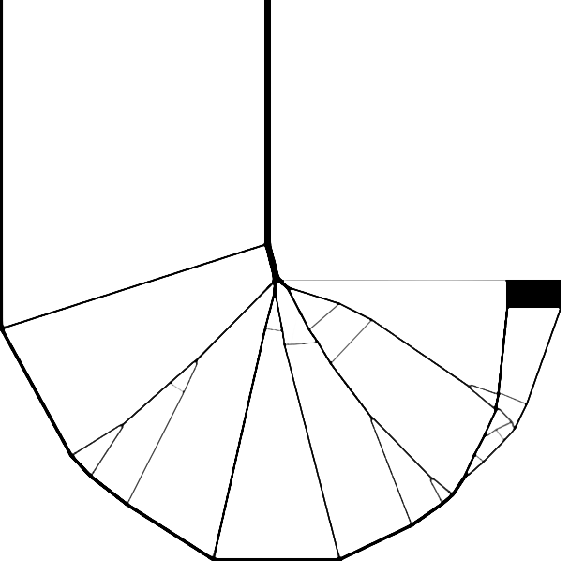
\includegraphics[width=0.23\linewidth ]{figures/03_comparison_TO_TTO/05_to_sol/fig0_2.pdf}}
    \hfill
    \subcaptionbox{}{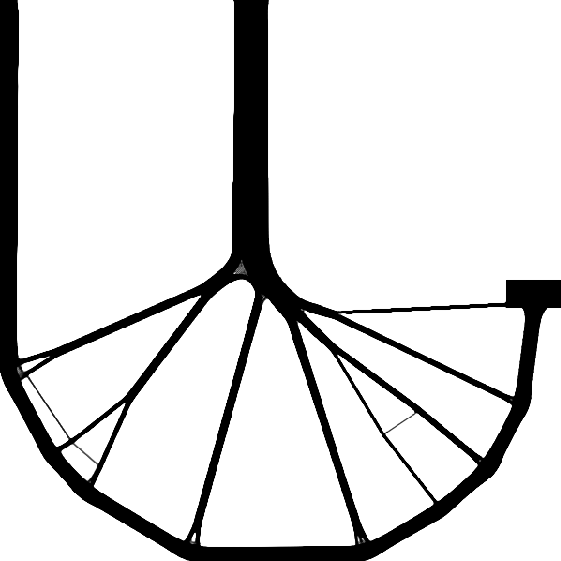
\includegraphics[width=0.23\linewidth ]{figures/03_comparison_TO_TTO/05_to_sol/fig0_0.4.pdf}}
    \hfill
    \subcaptionbox{}{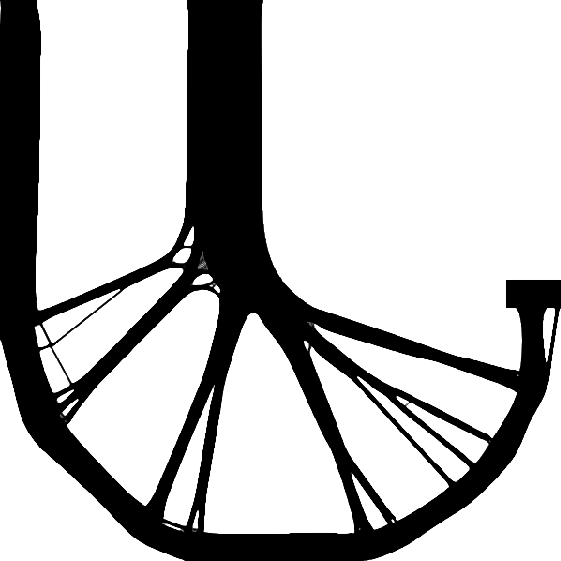
\includegraphics[width=0.23\linewidth ]{figures/03_comparison_TO_TTO/05_to_sol/fig0_0.25.pdf}}
    \bigskip
    \subcaptionbox{}{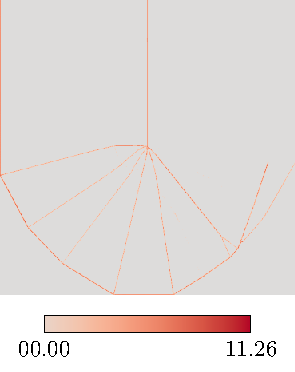
\includegraphics[width=0.23\linewidth ]{figures/03_comparison_TO_TTO/05_to_sol/stress_10.pdf}}
    \hfill
    \subcaptionbox{}{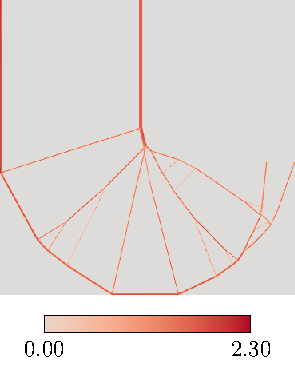
\includegraphics[width=0.23\linewidth ]{figures/03_comparison_TO_TTO/05_to_sol/stress_2.pdf}}
    \hfill
    \subcaptionbox{}{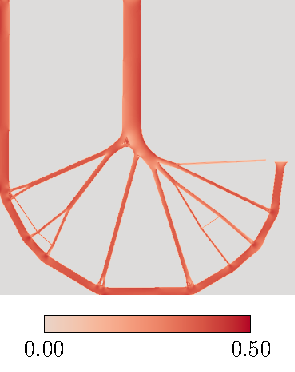
\includegraphics[width=0.23\linewidth ]{figures/03_comparison_TO_TTO/05_to_sol/stress_04.pdf}}
    \hfill
    \subcaptionbox{}{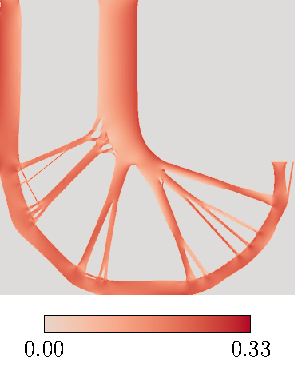
\includegraphics[width=0.23\linewidth ]{figures/03_comparison_TO_TTO/05_to_sol/stress_025.pdf}}
    \caption{\todo{todo}}
    \label{fig:03_to_sol}
\end{figure*}
In this section we generate multiple optimized structures with diferent volume fractions $V_\text{f}$ by launching the optimization code for continuous mesh with different values of the material admissible $\sigma_\text{L}$ spanning from $0.2$ to $20$.

On top of volume fraction, compliance and stress, we evaluate an additional metric \todo{propre au maillage continu} called the \textit{measure of non-discreteness}~\sidecite{sigmund_morphology-based_2007} to evaluate the quality of the solutions. It is defined as:
\begin{equation}
    M_\text{nd} = \frac{\sum_e 4 \rhophys_e(1-\rhophys_e)}{n} \times 100 \%,
\end{equation}
where results near-zero mean a completely black and white design. 

The results obtained for $\sigma_\text{L}=10.00,2.00,0.40\text{ and }0.25$ are shown in \figref{fig:03_to_sol}. In the upper part of the figure we see the topology of the optimized structures with a clearly ascending volume fraction $V_\text{f}$. Interestingly, the topology of the solution remains almost unchanged, varying principally the thickness of his members. We notice the classic large fillet around the corner that alleviate the stress concentration problem. As the volume decrease, the optimized structure tend to a solution that ressemble Michell structures. In those cases we know that the topology optimization algorithm act like a method for layout of truss-like structures~\sidecite{bendsoe_generating_1988}. This effect is caused by the combination of different factors, as the regularization filter, the mesh size and the low volume fraction~\sidecite{sigmund_non-optimality_2016}. A summary of the numerical results is presented in \tabref{tab:TO_results}.

In the lower part of \figref{fig:03_to_sol}, we plot the equivalent Von Mises stress for every element of the solution with pysical density $\rhophys>0.5$. Multiple interesting observations can be made. First, we notice that the stress distribution is almost uniform in the structure, and it tend to the value of the material admissible $\sigma_\text{L}$ -- \ie we approach a \textit{fully stressed} structure. Even if the geometric support of the teory are different, it looks like the topology optimized structures follows the Michell criteria presented in \secref{sec:03_michell} for optimal truss structures. Furthermore, it is observed that the maximum stress exceeds the material admissible $\sigma_\text{L}$. Aggregation methods aim to estimate the maximum value of the stress constraint across a group of elements. However, these aggregation methods do not perfectly align with the exact maximum value, which is a recognized limitation. To address this challenge, multiple approaches have been proposed within the aggregation framework to accurately account for the true constraint value, like using a set of active stress constraints~\sidecite{bruggi_topology_2012}, several aggregation clusters~\sidecite{paris_block_2010} or rectifier functions~\sidecite{norato_maximum-rectifier-function_2022}.

Looking again at \tabref{tab:TO_results}, we notice that the optimization processes exhibit prolonged execution times, especially when dealing with extreme cases like high volume fractions. This effect is likely caused by the very fine mesh used to discretize the design domain $\Omega$ and by the sensitivity calculation by the means of the adjoint method.

\begin{table}[]
    \centering
    \sisetup{table-auto-round}
    \begin{tabular}{S[table-format = 2.2]
                    S[table-format = 2.2]
                    S[table-format = 2.2]
                    S[table-format = 5.0]
                    S[table-format = 1.2]
                    S[table-format = 4.0]
                    c
                    }
    \toprule
    $\bm \sigma_L$ & $\bm \max \bm \sigma_L$   & $\bm V_\text{f}$     & $\bm C$ & $M_\text{nd}$  & {\textbf{It.}}  & {\textbf{Time}}      \\ \midrule
    20    & 23.51 & 1.18       & 6992.10    & \qty{1.91}{\percent} & 1142     & $\hms{08;11;00}$ \\
    10    & 11.26 & 1.60       & 3837.08    & \qty{2.19}{\percent} & 1147     & $\hms{07;55;00}$ \\
    8     & 8.78  & 1.74       & 2765.60    & \qty{1.95}{\percent} & 792      & $\hms{05;39;00}$ \\
    6     & 7.15  & 1.89       & 2243.31    & \qty{1.81}{\percent} & 806      & $\hms{05;35;00}$ \\
    5     & 5.81  & 2.17       & 1823.12    & \qty{1.81}{\percent} & 849      & $\hms{05;53;00}$ \\
    4     & 4.69  & 2.67       & 1423.54    & \qty{2.02}{\percent} & 894      & $\hms{06;12;00}$ \\
    3     & 3.47  & 3.00       & 1132.79    & \qty{1.64}{\percent} & 993      & $\hms{06;45;00}$ \\
    2     & 2.30  & 4.04       & 781.48     & \qty{1.45}{\percent} & 1189     & $\hms{08;20;00}$ \\
    1     & 1.18  & 7.28       & 403.53     & \qty{1.35}{\percent} & 1621     & $\hms{11;41;00}$ \\
    0.90  & 1.06  & 8.09       & 364.80     & \qty{1.31}{\percent} & 1656     & $\hms{11;36;00}$ \\
    0.80  & 0.96  & 8.82       & 331.95     & \qty{1.21}{\percent} & 1937     & $\hms{15;21;00}$ \\
    0.70  & 0.84  & 10.05      & 291.89     & \qty{1.09}{\percent} & 1827     & $\hms{13;21;00}$ \\
    0.60  & 0.73  & 11.80      & 250.23     & \qty{1.19}{\percent} & 1955     & $\hms{14;21;00}$ \\
    0.50  & 0.61  & 14.18      & 213.01     & \qty{1.06}{\percent} & 2032     & $\hms{15;39;00}$ \\
    0.40  & 0.50   & 18.03      & 169.90     & \qty{1.08}{\percent} & 2259     & $\hms{17;06;00}$ \\
    0.35  & 0.44  & 21.12      & 148.13     & \qty{1.15}{\percent} & 2421     & $\hms{19;29;00}$ \\
    0.30  & 0.38  & 26.21      & 125.69     & \qty{1.50}{\percent} & 3100     & $\hms{24;46;00}$ \\
    0.25  & 0.33  & 34.71      & 104.30     & \qty{1.04}{\percent} & 3484     & $\hms{27;39;00}$ \\
    0.20  & 0.27  & 48.08      & 76.56      & \qty{1.26}{\percent} & \color{accent_r_1}7500     & $\hms{91;46;00}$ \\ \bottomrule
    \end{tabular}
    \caption{TO}
    \label{tab:TO_results}
    \end{table}
    
\begin{marginfigure}
        \centering
        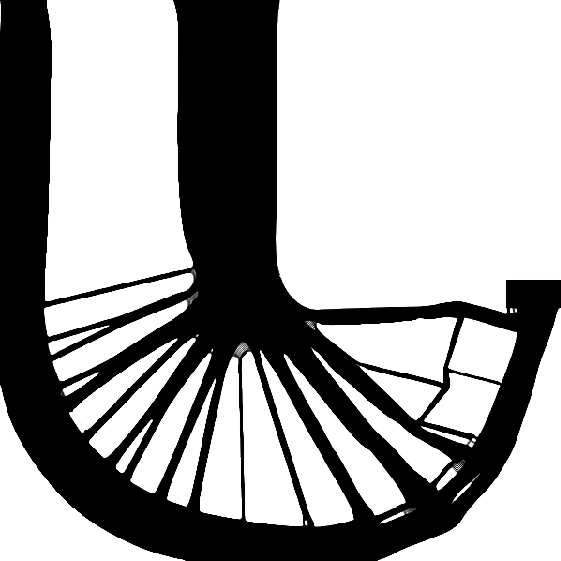
\includegraphics[width=0.8\linewidth]{figures/03_comparison_TO_TTO/06_to_no/fig0.pdf}
        \caption{\todo{add mnd}}
        \label{fig:03_to_sol_no}
    \end{marginfigure}

As previously mentioned, our focus lies in exploring the method's limits, particularly at the boundaries. When dealing with excessively weak materials, we encounter a scenario where no solution can be attained since no distribution can simultaneously fulfill the imposed constraints. Throughout our research with this specific test case and mesh size, we did not produce any solutions with a volume fraction exceeding 50\%. Although we haven't reached that scenario with $\sigma_\text{L}$ set to 0.2, the calculation time and the number of iterations increase significantly, we have encountered the method's limits. The calculation time has significantly increased because the algorithm faces greater difficulty in satisfying the stress constraints. \figref{fig:03_to_sol_no} shows the topology of the solution with $\sigma_\text{L}=0.2, \; V_\text{f}=48.08\%$ and over five days of optimization.

\begin{marginfigure}
    \centering
    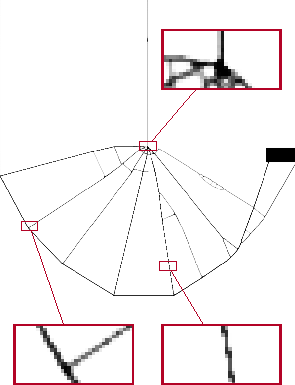
\includegraphics[width=0.8\linewidth]{figures/03_comparison_TO_TTO/00_to_zoom/to_zoom.pdf}
    \caption{\todo{todo}}
    \label{fig:03_to_sol_zoom}
\end{marginfigure}
Conversely, when dealing with an exceedingly strong material, the optimal scenario would demand such minimal material usage that certain sections of the structure become thinner than the width of a single element. In this case, the mesh used for discretization is too coarse to accurately represent the solution, and finer meshing becomes essential to capture the intricate details of the optimized design. \figref{fig:03_to_sol_zoom} shows
the limit case when $\sigma_\text{L}=10.0$ and $ V_\text{f}=1.60\%$ \todo{pulisci grafici e tabella dai risultati fuori dai limiti}

Finally, in \figref{fig:03_to_plot} are the plots summarizing our findings, with the limits highlighted. To effectively show the different orders of magnitude present in the plot, we have used both linear and logarithmic scales simultaneously.
\begin{figure*}[]
    \hspace*{\fill}
    \subcaptionbox{\label{fig:03_to_plot_lin}}{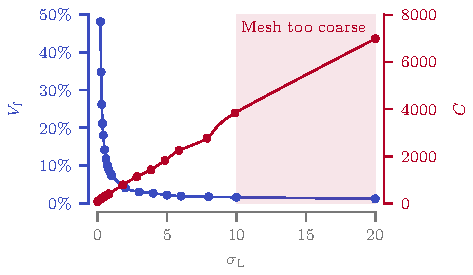
\includegraphics{figures/03_comparison_TO_TTO/07a_to_graph_lin/to_c_lin.pdf}}
    \hfill
    \subcaptionbox{\label{fig:03_to_plot_log}}{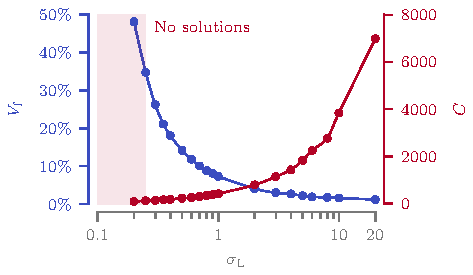
\includegraphics{figures/03_comparison_TO_TTO/07b_to_graph_log/to_c.pdf}}
    \hspace*{\fill}
    \caption{}
    \label{fig:03_to_plot}
\end{figure*}
It's interesting to note that the volume fraction $V_\text{f}$ follows a hyperbolic relationship, while compliance $C$ exhibits a linear correlation with respect to the material admissible $\sigma_\text{L}$.

\paragraph{Truss mesh optimization results}
we present here the results of the truss discretization. hre in fig the topology and the stress of the solutions for every stress limit. as formulation P0 with the L test case and simmetric stress constraints respect the michell crtiteria the solution  topology is the same and it is fully stressed.

\begin{figure}[]
    \centering
    \hspace*{\fill}
    \subcaptionbox{\label{fig:03_tto_sol_tc}}{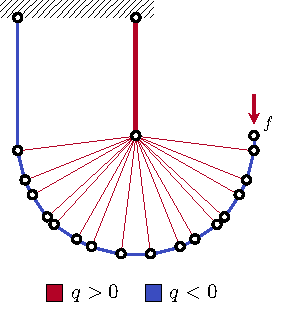
\includegraphics[valign=t]{figures/03_comparison_TO_TTO/05_tto_sol/L_tto_opt.pdf}}
    \hfill
    \subcaptionbox{\label{fig:03_tto_sol_st}}{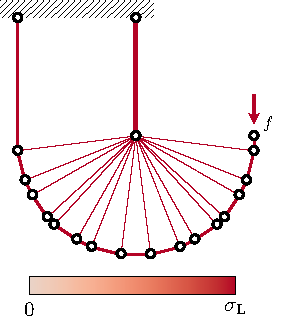
\includegraphics[valign=t]{figures/03_comparison_TO_TTO/05_tto_sol/L_tto_opt_st.pdf}}
    \hspace*{\fill}
    \caption{testtesttest}
    \label{fig:03_L_tto}
\end{figure}
\begin{equation}
    PL/\sigma
\end{equation}\sidecite{lewinski_extended_1994} is constant

the execution time is on the order of 60 s. full results are availabe in table ..

\begin{table}[]
    \centering
    \sisetup{table-auto-round}
    \begin{tabular}{S[table-format = 2.1]
                    S[table-format = 2.2]
                    S[table-format = 5.0]
                    S[table-format = 2.1]                    
                    S[table-format = 2.0]}
        
    \toprule
    $\bm \sigma_L$ & $\bm V_\text{f}$     & $\bm C$      & {\textbf{Min} $\bm \lambda$} & {\textbf{Time}} \\ \midrule
    50         & 0.124169  & 23281.62 & 111.687                     & $\hms{00;01;06}$    \\
    20         & 0.310422  & 9312.65  & 70.637                      & $\hms{00;01;09}$    \\
    10         & 0.620843  & 4656.32  & 49.948                      & $\hms{00;01;18}$    \\
    8          & 0.776054  & 3725.06  & 44.675                      & $\hms{00;01;15}$    \\
    6          & 1.034739  & 2793.79  & 38.689                      & $\hms{00;01;10}$    \\
    5          & 1.241686  & 2328.16  & 35.318                      & $\hms{00;01;24}$    \\
    4          & 1.552108  & 1862.53  & 31.590                      & $\hms{00;01;18}$    \\
    3          & 2.069477  & 1396.90  & 27.358                      & $\hms{00;01;15}$    \\
    2          & 3.104216  & 931.26   & 22.337                      & $\hms{00;01;15}$    \\
    1          & 6.208431  & 465.63   & \color{accent_r_2}15.795    & $\hms{00;01;17}$    \\
    0.90       & 6.898257  & 419.07   & \color{accent_r_2}14.984    & $\hms{00;01;20}$    \\
    0.80       & 7.760539  & 372.51   & \color{accent_r_1}14.127    & $\hms{00;01;21}$    \\
    0.70       & 8.869187  & 325.94   & \color{accent_r_1}13.215    & $\hms{00;01;16}$    \\
    0.60       & 10.347385 & 279.38   & \color{accent_r_1}12.235    & $\hms{00;01;20}$    \\
    0.50       & 12.416862 & 232.82   & \color{accent_r_1}11.169    & $\hms{00;01;22}$    \\
    \bottomrule    
    \end{tabular}
    \caption{TTO}
    \label{tab:TTO_results}
    \end{table}

dire che visto il test di convergenza suiulla mesh della TO prendiamo una mesh qui 33x33 ma che in realta il risutato buono ce lo abbiamo anche gia soltanto a 13x 13 con tempo di calcolo irrisorio
\begin{marginfigure}
    \centering
    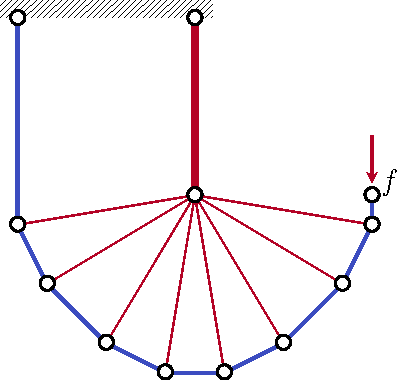
\includegraphics[width=0.8\linewidth]{figures/03_comparison_TO_TTO/05b_tto_sol_13/L_tto_opt.pdf}
    \caption{\todo{todo}}
    \label{fig:03_L_tto_13}
\end{marginfigure}

To explore telimit of the method we look at the boundary. in order to evaluate the quality we use a different metric
segna da qualche parte la slenderness maximum
minimum slenderness ratio $\lambda$ (ratio between the length and the radius of gyration of the bar) of a bar is

the compliance is linear and the volume is hyperbolic exactly

\begin{figure*}[]
    \hspace*{\fill}
    \subcaptionbox{\label{fig:03_tto_plot_lin}}{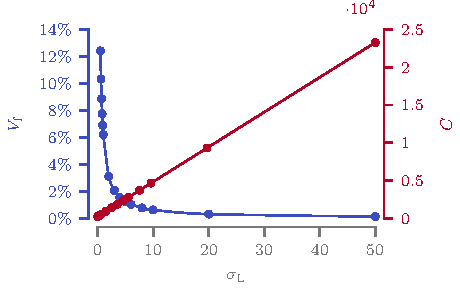
\includegraphics{figures/03_comparison_TO_TTO/07a_tto_graph_lin/tto_c_lin.pdf}}
    \hfill
    \subcaptionbox{\label{fig:03_tto_plot_log}}{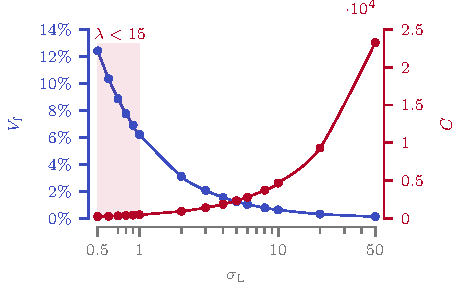
\includegraphics{figures/03_comparison_TO_TTO/07b_tto_graph_log/tto_c.pdf}}
    \hspace*{\fill}
    \caption{}
    \label{fig:03_tto_plot}
\end{figure*}

\subsection{Discussion}
We present here the comparison graph of the two formulations
the graphs are trimmed to their limits
\paragraph{Stress-compliance graph}
\begin{figure}[]
    \centering
    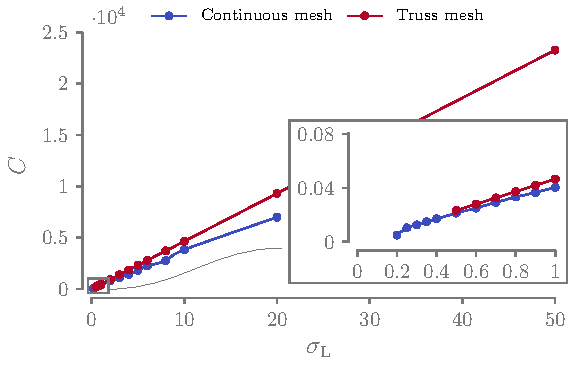
\includegraphics{figures/03_comparison_TO_TTO/00_stress_comp/stress_comp.pdf}
    \caption{\todo{caption}}
    \label{fig:03_stress_comp}
\end{figure}
the truss is always less compliant and linear

\paragraph{Stress-volume graph}
\begin{figure}[]
    \centering
    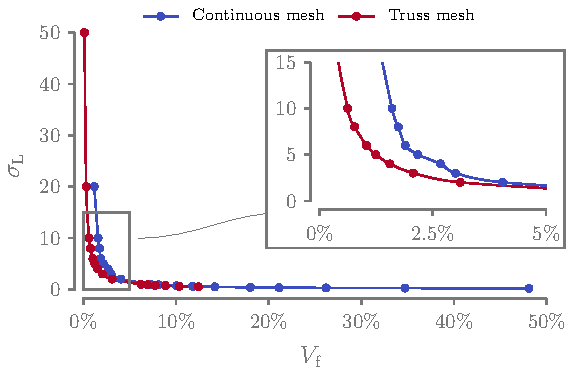
\includegraphics{figures/03_comparison_TO_TTO/00_stress_vol/stress_vol.pdf}
    \caption{\todo{caption}}
    \label{fig:03_stress_vol}
\end{figure}
The TO generate structures that for a given material admissible are more massive. scrivi che la differenza ad alti volumi viene dal fatto che c'é un cap allo spessore massimo nella TO

interesting that the 
the truss representation is the bourne inferieur de la TO for low volume fraction, while interestingly the two discretization follows the same allure for high volume fractions despite the big pysical description difference

\paragraph{Volume-compliance graph}
\begin{figure}[]
    \centering
    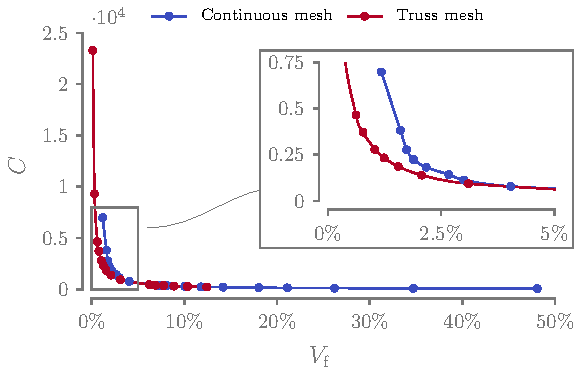
\includegraphics{figures/03_comparison_TO_TTO/00_comp_vol/comp_vol.pdf}
    \caption{\todo{caption}}
    \label{fig:03_comp_vol}
\end{figure}


\todo{fai check che tutti i dati nella comparison abbiano senso e riempi i dati con il 50}

finally we observe the time comparison time comparison

\begin{figure}[]
    \centering
    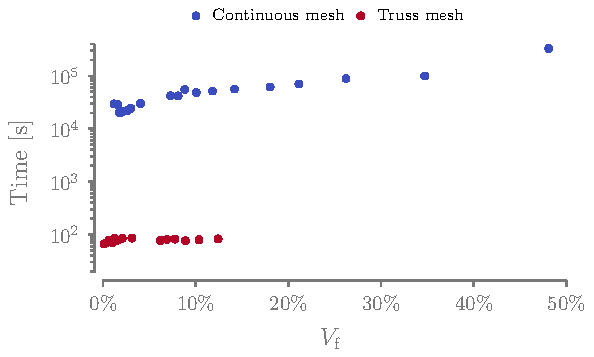
\includegraphics{figures/03_comparison_TO_TTO/00_time_vol/time_vol.pdf}
    \caption{\todo{caption}}
    \label{fig:03_time_vol}
\end{figure}

When stress no self adjoint \gls{sand} could be benificial however to add more constraints such as stress buckling and displacements because in that way no self adjoint

calculation time for the double of opt variables, open up the way toward sand topopt One should consider that \gls{sand} approaches usually increases the number of design variables considerably. Nevertheless, in truss topology problems this is less concerning, as the ground structure approach results in numerous cross-sectional area design variables and fewer displacement-related ones. This, however, does not hold true when dealing with a continuous mesh, where the \gls{nand} approach reduces considerably the number of design variables.

additionally interesting how the solution is not influenced by the number of nodes. expecially at low volume fration vs TO that needs more an more elements the finer we want to go

other limits of the continuous discretizations

cita l'overshoot dello stress, risolvibile ma a patto di aumentare ancora il tempo di calcolo

buckling definition is easier on truss modeled

parla del fatto che é difficile essere asimmetrico in topopt

so we select the tto

problems of the tto (open to the new chapter)
in min vol the problem is linear and unexpensive to solve, but that is not always the case if we add buckling, multiload
explain the problem of compatibility quick

\section{Conclusion}
"We noted that the analytical models of the isotruss and octet truss in the literature are accurate at low relative densities, but lose their accuracy for higher relative densities. Relative errors of 10\% in the elastic moduli existed at all relative densities greater than approximately 2\%."~\sidecite{watts_simple_2019}
"The methods allow for a determination of the topology of a mechanical element and give useful information on the form of the boundaries of the optimal shape. For moderately low volume fractions the lay-out of truss-like structures is predicted, but for very low volume fractions it is recommended that the traditional lay-out theory be employed, as described by Rozvany (1984)."~\sidecite{bendsoe_optimal_1989}

but the performance gap has never been mesurated nor the domain of appicability. here's wy of this chapter. on the top of that these assumptions where on complaince formulations
we have introduced the formulation
we have run the analysis on a common load case
we have compared the results
we have selected the truss topology optimization
BUT
Open to the new chapter
